%% Lab Report for EEET2493_labreport_template.tex
%% V1.0
%% 2019/01/16
%% This is the template for a Lab report following an IEEE paper. Modified by Francisco Tovar after Michael Sheel original document.


%% This is a skeleton file demonstrating the use of IEEEtran.cls
%% (requires IEEEtran.cls version 1.8b or later) with an IEEE
%% journal paper.
%%
%% Support sites:
%% http://www.michaelshell.org/tex/ieeetran/
%% http://www.ctan.org/pkg/ieeetran
%% and
%% http://www.ieee.org/

%%*************************************************************************
%% Legal Notice:
%% This code is offered as-is without any warranty either expressed or
%% implied; without even the implied warranty of MERCHANTABILITY or
%% FITNESS FOR A PARTICULAR PURPOSE! 
%% User assumes all risk.
%% In no event shall the IEEE or any contributor to this code be liable for
%% any damages or losses, including, but not limited to, incidental,
%% consequential, or any other damages, resulting from the use or misuse
%% of any information contained here.
%%
%% All comments are the opinions of their respective authors and are not
%% necessarily endorsed by the IEEE.
%%
%% This work is distributed under the LaTeX Project Public License (LPPL)
%% ( http://www.latex-project.org/ ) version 1.3, and may be freely used,
%% distributed and modified. A copy of the LPPL, version 1.3, is included
%% in the base LaTeX documentation of all distributions of LaTeX released
%% 2003/12/01 or later.
%% Retain all contribution notices and credits.
%% ** Modified files should be clearly indicated as such, including  **
%% ** renaming them and changing author support contact information. **
%%*************************************************************************

\documentclass[journal]{IEEEtran}

% *** CITATION PACKAGES ***
\usepackage[style=ieee]{biblatex} 
\bibliography{example_bib.bib}    %your file created using JabRef

% *** MATH PACKAGES ***
\usepackage{amsmath}
\usepackage{amsfonts}
\usepackage{comment}
\usepackage{amssymb} % Este paquete contiene el símbolo \approxeq

\usepackage{tabularx} % en el preámbulo
\usepackage{caption}
\captionsetup{font=small, labelfont=bf, textfont=normalfont}


% *** PDF, URL AND HYPERLINK PACKAGES ***
\usepackage{url}
% correct bad hyphenation here
\hyphenation{op-tical net-works semi-conduc-tor}
\usepackage{graphicx}  %needed to include png, eps figures
\usepackage{subcaption}
\usepackage{float}  % used to fix location of images i.e.\begin{figure}[H]

\begin{document}

% paper title
\title{Fuente Bipolar Lineal\\ \small{Proyecto No. 1}}

% author names and affiliations
\author{
    \IEEEauthorblockN{Flores Cornejo Gustavo Mauricio, Muñoz Reyes Arturo Yabed, Morales Vásquez Miguel Ehecatl}\\
    \IEEEauthorblockA{\textit{Unidad Profesional Interdisciplinaria en Ingeniería y Tecnologías Avanzadas, IPN}}
}
        
% The report headers
\markboth{1MV12 Fundamentos de Electrónica. Proyecto 1, Abril 2026}%do not delete next lines
{Shell \MakeLowercase{\textit{et al.}}: Bare Demo of IEEEtran.cls for IEEE Journals}

% make the title area
\maketitle

% As a general rule, do not put math, special symbols or citations
% in the abstract or keywords.
\begin{abstract}
    This project details the development of a linear bipolar power supply designed to provide regulated positive 
    and negative voltages. The process begins with mathematical sizing based on the nominal values of a center-tapped 
    transformer, followed by a rectification stage and the calculation of filter capacitors to ensure a ripple voltage of less than 10\%
    of the DC level. A regulation scheme was implemented using 78XX and 79XX integrated circuits, with specific load resistors 
    calculated to evaluate the system at 75\% of its rated current. Experimental results, obtained through the use of an 
    oscilloscope and a multimeter, demonstrate that the design meets the proposed regulation and stability criteria, validating 
    the design methodology against the manufacturer's technical data.
\end{abstract}

\section{Introducción}
    % Here we have the typical use of a "W" for an initial drop letter
    % and "RITE" in caps to complete the first word.
    % You must have at least 2 lines in the paragraph with the drop letter
    % (should never be an issue)

    \IEEEPARstart{L}as fuentes de alimentacion han sido un pilar fundamental en el diseño de sistemas electricos, donde la estabilidad
    y fidelidad de la tensión de corriente directa (CD) son determinantes para el rendimiento y la integridad de los componentes. 
    En el contexto de la infraestructura eléctrica convencional, es necesario transformar la tensión de corriente alterna (CA), 
    proveniente de la red de distribución, en niveles de CD regulados que permitan el funcionamiento de dispositivos electrónicos de uso cotidiano e industrial.
    
    El presente reporte documenta el proceso integral de diseño, construcción y validación de una fuente de alimentación 
    bipolar lineal fundamentada en reguladores integrados de las series 78XX y 79XX. El análisis técnico abarca desde la 
    etapa de rectificación de onda completa y el dimensionamiento del filtrado capacitivo, hasta la etapa de regulación 
    de voltaje bajo condiciones de carga controlada. Se pone especial énfasis en asegurar que parámetros críticos, 
    como el voltaje de rizo (limitado a un máximo del 10\% de la CD) y la regulación de voltaje, cumplan estrictamente con los estándares 
    de diseño propuestos y las especificaciones técnicas proporcionadas en las hojas de datos del fabricante.

\section{Objetivos}
    \subsection{Objetivo General}
    Diseñar y construir experimentalmente una fuente de alimentación bipolar lineal 
    empleando reguladores integrados 78XX y 79XX, garantizando un suministro eléctrico estable y 
    simétrico para aplicaciones electrónicas de baja potencia.

    \subsection{Objetivos Particulares}
    \begin{enumerate}
        \item Calcular y dimensionar los componentes críticos del sistema (capacitores de filtro y resistencias de carga) bajo criterios de diseño que limiten el voltaje de rizo a un máximo del 10\%.
        \item Verificar mediante instrumentación (multímetro y osciloscopio) que los voltajes de salida y los niveles de rizo se mantengan dentro de los márgenes de operación nominales bajo condiciones de carga al 75\% de la capacidad del circuito integrado.
        \item Evaluar el porcentaje de regulación de voltaje del sistema para comparar el desempeño experimental frente a las características típicas especificadas por el fabricante en las hojas de datos.
    \end{enumerate}

\section{Marco teórico}
    \subsection{Fuente de alimentación lineal}
        Una fuente de alimentación lineal es un sistema diseñado para convertir una tensión elevada de 
        corriente alterna (CA) en una tensión estabilizada de corriente directa (CD). Su nombre proviene del
        funcionamiento de sus componentes activos, a diferencia de las fuentes conmutadas, los reguladores
        ajustan su conducción para dicipar el exeso de energía en forma de calor. Este sistema se compone 
        de cinco etapas principales, las cuales son ejemplificadas en la Figura \ref{fig:diagrama_fuente} 
        por medio de un diagrama de bloques donde se aprecian los distintos niveles de voltaje en cada etapa. 

        \begin{figure}[H]%[!ht]
            \centering
            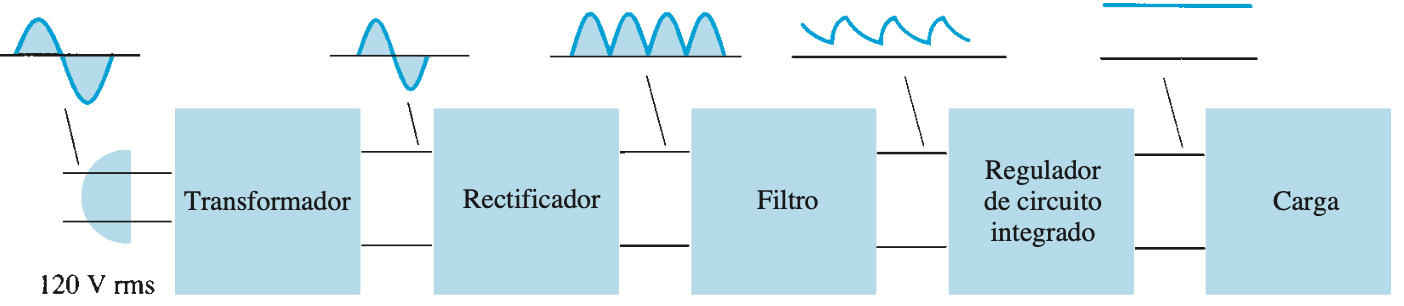
\includegraphics[width=0.48\textwidth]{IMAGENES/Diagrama_fuente.png}
            \caption{Diagrama de bloques que muestra las partes de una fuente de alimentación, tomado de Boylestad [1].}
            \label{fig:diagrama_fuente}
        \end{figure}
       
    \subsection{Transformador}
        El proceso inicia en el transformador, un dispositivo basado en la inducción electromagnética que reduce
        el nivel de tensión de la red eléctrica al valor requerido por el diseño. Es un factor crítico de diseño 
        considerar los parámetros de la red de suministro según la región geográfica. En la mayor parte de América, 
        el valor nominal es de 127 V rms a 60 Hz, mientras que en regiones como Europa y Oceanía, el estándar oscila entre 220-240 V rms a 50 Hz.
        Asi mismo, debe considerarse un voltaje de salida del debanado secundario que sea adecuado para los fines de la fuente y la carga.

    \subsection{Rectificador de onda completa}
        Una vez que el voltaje ha sido reducido por el transformador, la señal de CA debe convertirse en una señal unidireccional. 
        Este proceso se lleva a cabo en la etapa de rectificación, donde se utiliza un rectificador de onda completa (cuatro diodos dispuestos en forma de puente)
        para asegurar que tanto el semiciclo positivo como el negativo de la onda senoidal contribuyan a la salida de corriente directa.
        
        Dado que la fuente desarrollada en este trabajo es de tipo bipolar, el puente de diodos debe ser conectado al transformador
        como se muestra en la Figura \ref{fig:Rectificador_diagrama}. De esta manera logramos suministrar simultáneamente tensiones de salida positivas y negativas con respecto a una referencia 
        común o tierra (GND). Esta configuración es posible gracias al aprovechamiento de la derivación central del transformador, la cual permite establecer un punto de 
        potencial cero a partir del cual se rectifican y regulan dos ramas independientes.
        \begin{figure}[H]%[!ht]
            \centering
            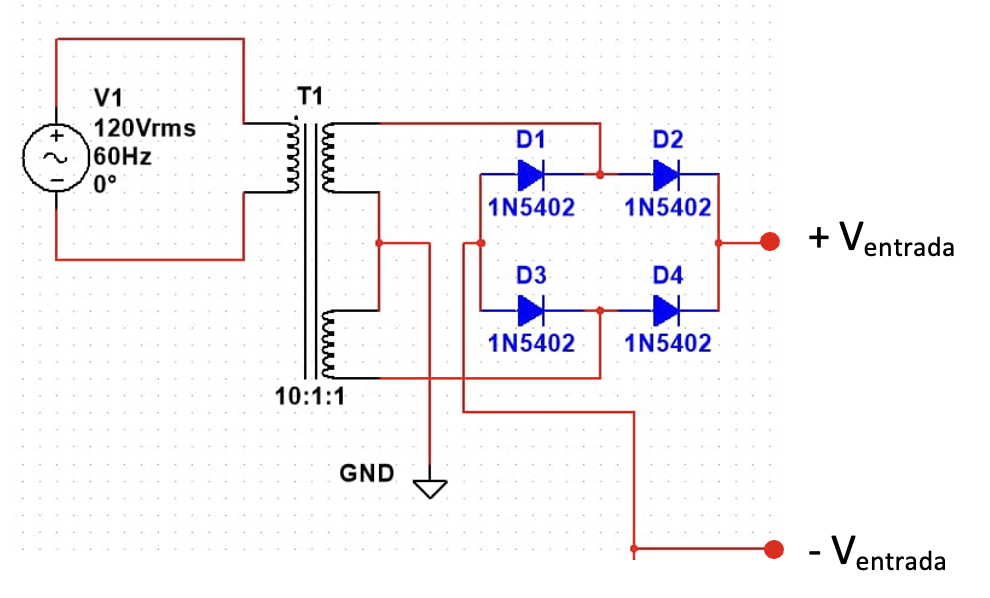
\includegraphics[width=0.45\textwidth]{IMAGENES/Rectificador_diagrama.png}
            \caption{Rectificador de onda completa con derivación central para dos tensiones de entrada a la carga.}
            \label{fig:Rectificador_diagrama}
        \end{figure}


    \subsection{Filtro Capacitivo}
    La salida del rectificador consiste en una serie de pulsos de voltaje que no son aptos para alimentar circuitos electrónicos sensibles. Para suavizar esta señal,
    se conecta un capacitor de filtro en paralelo. Este componente almacena energía durante el pico de voltaje y la libera cuando la señal del rectificador desciende,
    reduciendo significativamente las variaciones de tensión. El resultado es una señal de CD con un componente de corriente alterna residual conocido como voltaje de rizo ($V_{r}$).
    
    \subsection{Voltaje de rizo}
    De acuerdo con el análisis de Boylestad, el comportamiento del filtro capacitivo se define por dos intervalos críticos de operación dentro del ciclo de rectificación de onda completa, observese en Figura \ref{fig:Voltaje_rizo}. 
    En el primer intervalo ($T_1$), los diodos entran en conducción para cargar el capacitor hasta el valor de tensión pico ($V_m$). Posteriormente, durante el intervalo de descarga ($T_2$), 
    la tensión del rectificador decrece por debajo de $V_m$, obligando al capacitor a suministrar la energía almacenada a la carga. Dado que este ciclo se repite en cada semiciclo de la señal de entrada, 
    la frecuencia de la forma de onda resultante es el doble de la frecuencia de red ($2f$), lo que permite obtener un nivel de corriente directa ($V_{CD}$) con una componente de rizo residual ($V_r$) minimizada,
    cuya magnitud depende directamente de la constante de tiempo del circuito.s
        \begin{figure}[H]%[!ht]
            \centering
            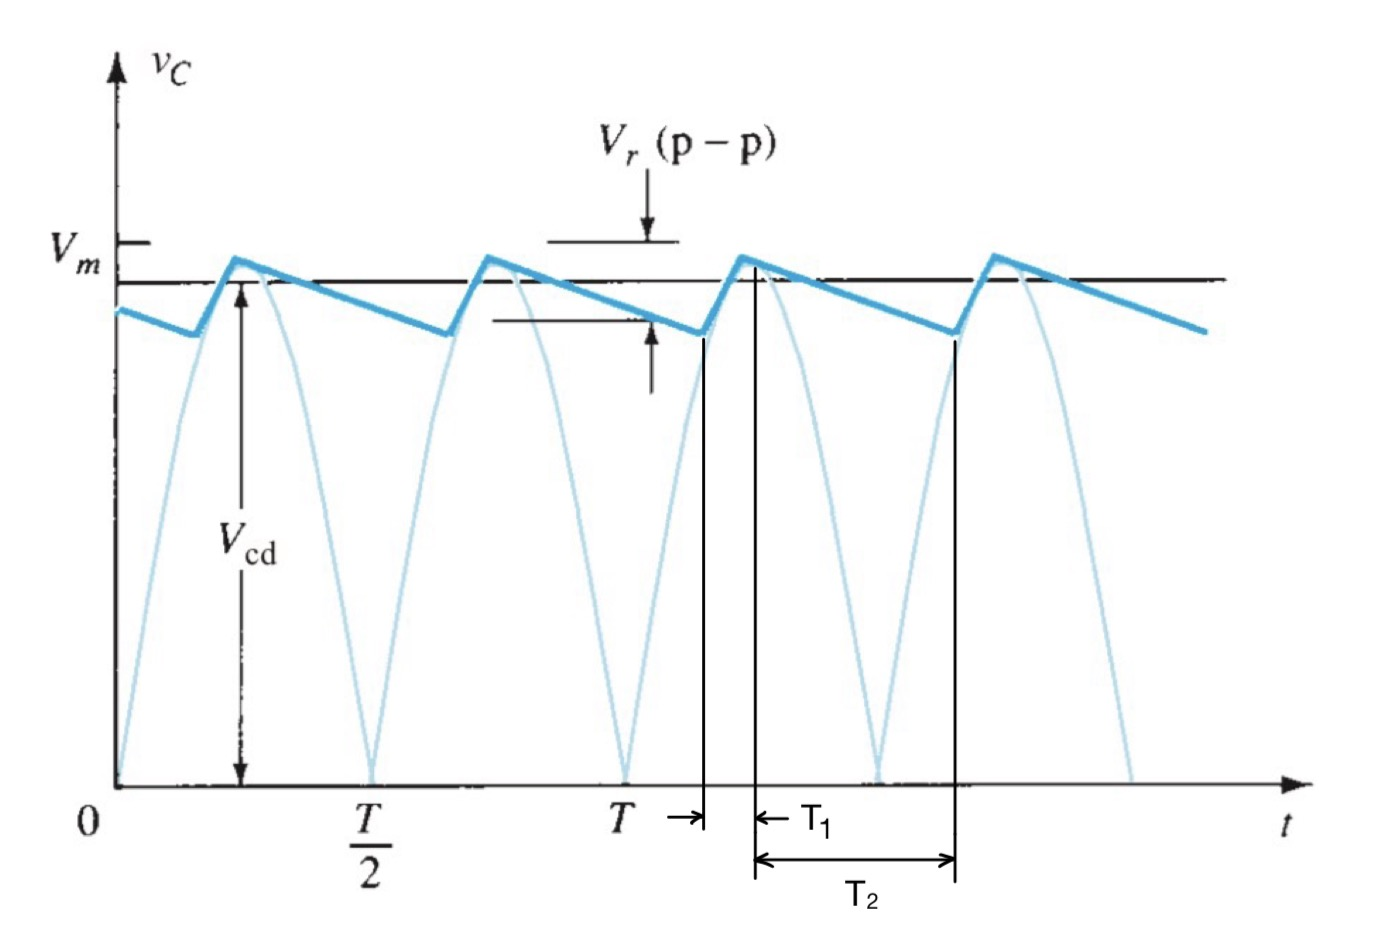
\includegraphics[width=0.45\textwidth]{IMAGENES/Voltaje_rizo.png}
            \caption{Voltaje de salida aproximado de un circuito de filtro de capacitor, modificado de Boylestad [1].}
            \label{fig:Voltaje_rizo}
        \end{figure}
        La relación entre el voltaje rizo y la capacitancia del capacitor esta dada por: 
        \begin{equation*}
            C = \frac{I_{carga}}{f \cdot V_{r\_(p-p)}}
        \end{equation*}
    \subsection{Corrientes de pico en el diodo}
    Como se menciono con anterioridad, en una configuración de filtrado capacitivo, la conducción del diodo se restringe exclusivamente al breve intervalo de tiempo ($T_1$) en el que el voltaje del secundario del transformador excede la tensión almacenada en el capacitor. Debido a que el condensador debe recuperar en este lapso toda la carga suministrada a la carga durante el resto del ciclo ($T_2$), la corriente fluye en forma de pulsos estrechos de gran magnitud conocidos como corrientes de pico. Como se observa en la Figura \ref{fig:formas_onda_diodo}, existe una relación crítica de diseño: a mayor capacitancia, menor será el ángulo de conducción y, consecuentemente, mayor será la intensidad del pico de corriente. Por tanto, es imperativo evitar el sobredimensionamiento excesivo de los capacitores, ya que, aunque reducen eficazmente el voltaje de rizo, pueden someter a los diodos a un estrés térmico que supere su capacidad de corriente de pico repetitivo ($I_{FRM}$), comprometiendo la integridad del rectificador.
    \begin{figure}[H]
        \centering
        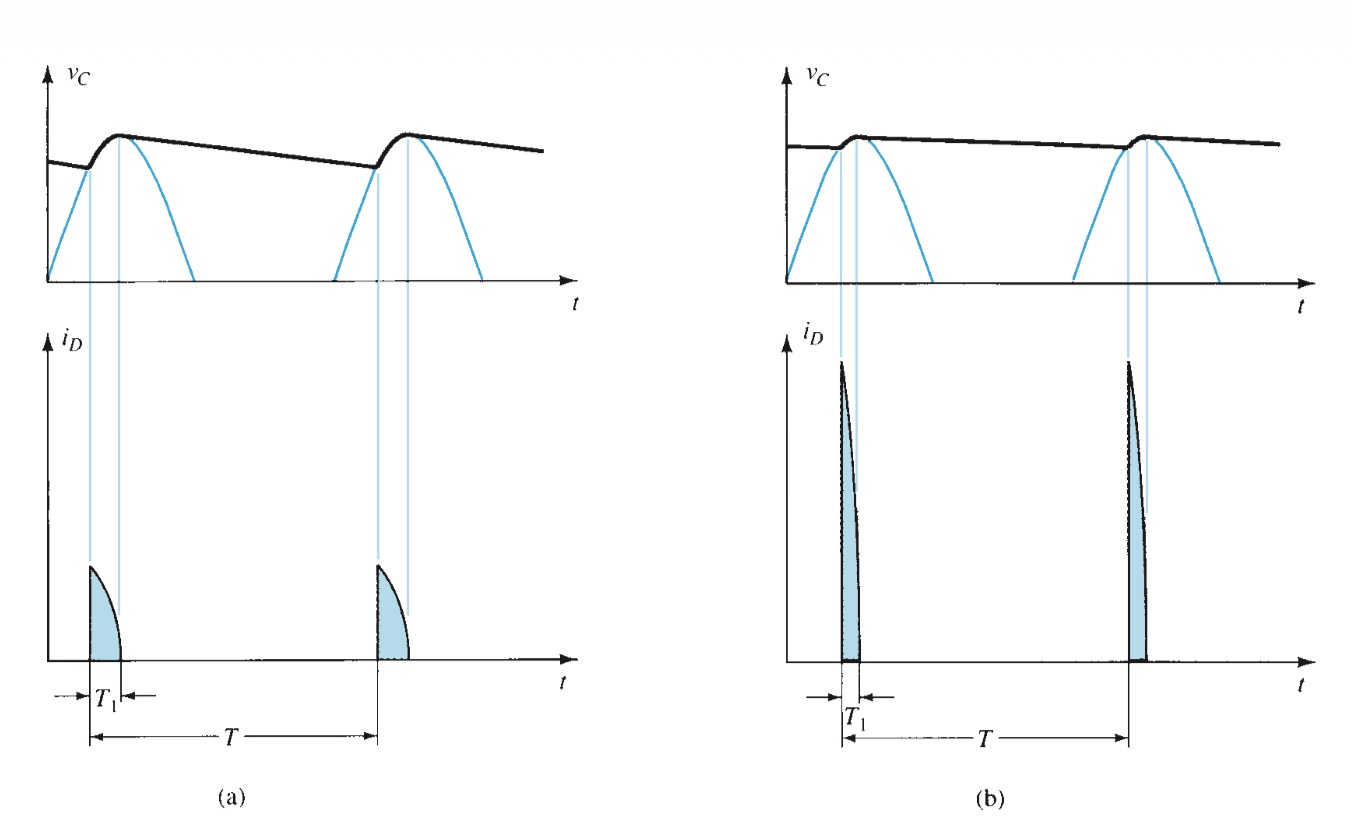
\includegraphics[width=0.48\textwidth]{IMAGENES/Corrientes_pico.png}
        \caption{Formas de onda del voltaje de salida (rizo) y de la corriente pulsante del diodo en un rectificador con filtro capacitivo, tomado de Boylestad [1].}
        \label{fig:formas_onda_diodo}
        \end{figure}

    \subsection{Regulación Lineal}
        La etapa final es la regulación, donde se emplean circuitos integrados de las familias 78XX (para voltajes positivos) y 79XX (para voltajes negativos). Estos dispositivos actúan de forma 
        analógica, ajustando su resistencia interna para mantener un voltaje de salida constante independientemente de las variaciones en la carga o en el voltaje de entrada. Para asegurar la 
        estabilidad del regulador, las hojas de datos del fabricante especifican la inclusión de capacitores de desacoplo en la entrada y salida del dispositivo, como se ilustra en la Figura \ref{fig:capacitores_regulador}.
        \begin{figure}[H]%[!ht]
            \centering
            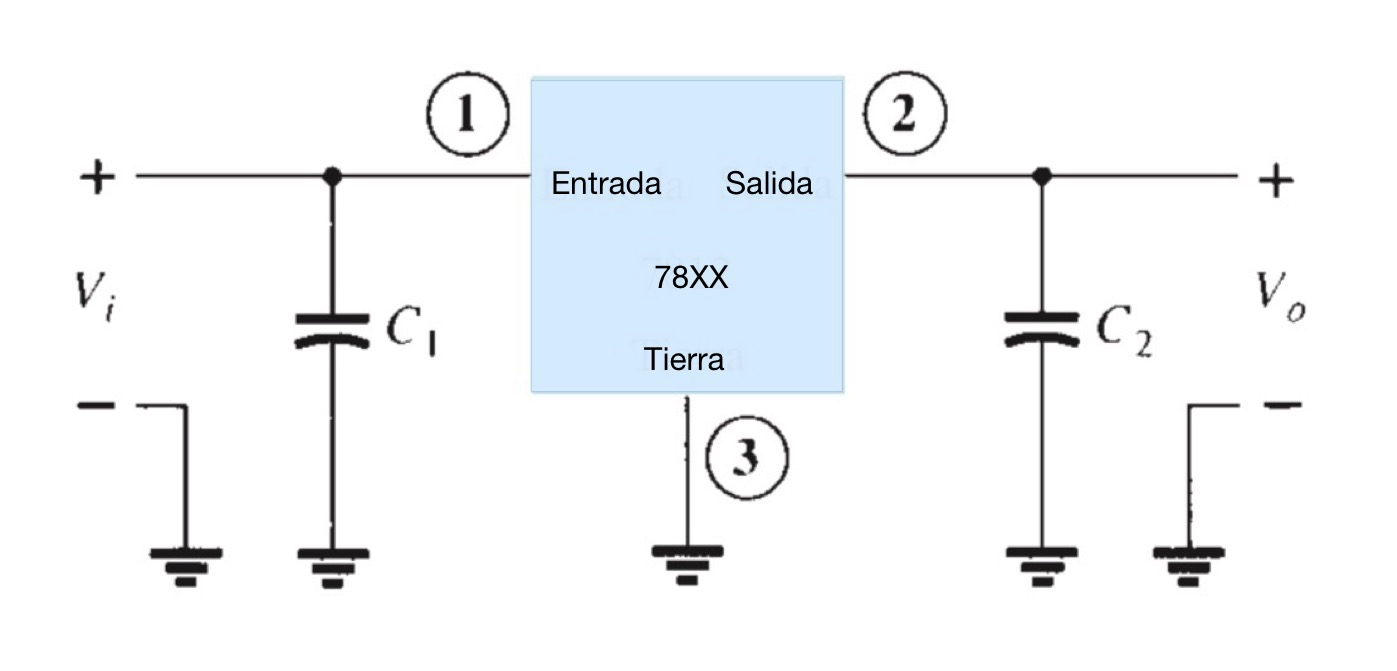
\includegraphics[width=0.45\textwidth]{IMAGENES/78XX_diagrama.png}
            \caption{Configuración recomendada por el fabricante para un regulador de la serie 78XX, modificado de Boylestad [1].}
            \label{fig:capacitores_regulador}
        \end{figure}
        Es de suma importancia respetar estos valores, ya que los parámetros de regulación y rechazo de rizo especificados en la hoja de datos se garantizan únicamente bajo estas condiciones de implementación.
    \subsection{Especificaciones de los Reguladores Integrados}
    El desempeño de los reguladores de las familias 78XX y 79XX está condicionado por parámetros fundamentales descritos en sus hojas de especificaciones. Entre estos destacan la tolerancia en el voltaje nominal de salida, la regulación de carga y las protecciones contra sobrecorriente. Un factor crítico de diseño es el \textit{dropout voltage} o voltaje de desconexión, el cual impone una diferencia mínima de potencial (típicamente 2 V) entre la entrada y la salida para asegurar un funcionamiento estable. Ignorar este margen resultaría en una pérdida de regulación, permitiendo que el rizo del capacitor se transfiera directamente a la carga.



    
\section{Materiales}
        \begin{figure} [H]
            \centering
            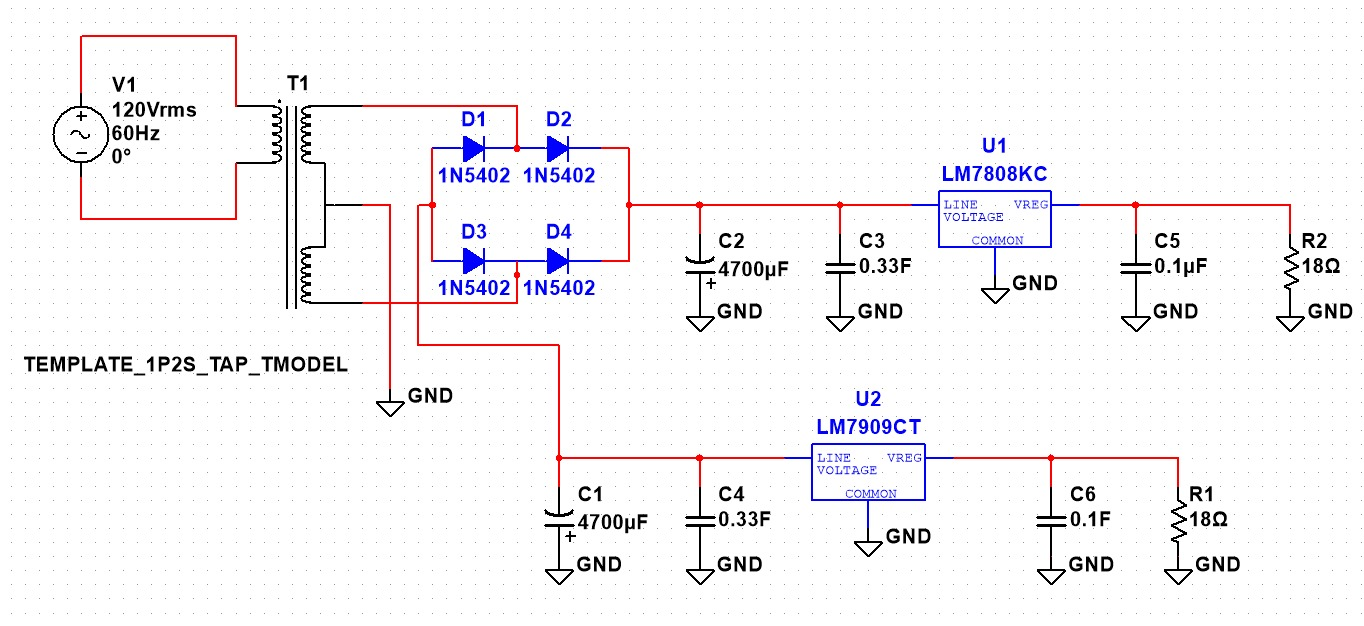
\includegraphics[width=0.4\textwidth]{IMAGENES/Circuito_base.jpeg}
            \caption{Circuito de fuente bipolar lineal.}
            \label{fig:circuito_base}
        \end{figure}
Para el circuito mostrado en la "Figura~\ref{fig:circuito_base}”, emplearemos:
\begin{itemize}
    \item 4 Diodos 1N5402.
    \item 1 Transformador 120 $V_{rms}$/24 $V_{rms}$ a 2A Y 60Hz.
    \item 2 Capcaitores Electrolíticos de 4700$\mu$F.
    \item 2 Capacitores Cerámicos de 0.33$\mu$F.
    \item 2 Capacitores Cerámicos de 0.10$\mu$F.
    \item 1 Regulador de Voltaje Lineal LM7809.
    \item 1 Regulador de Voltaje Lineal LM7909.
    \item 2 Resistencias de 18$\Omega$ a 10W.
\end{itemize}


\section{Análisis y Resultados}
Para el desarrollo de los cálculos utilizados para obtener los valores comerciales de cada componente del circuito anteriormente mostrado se procedió con las expresiones propuestas por el Boylestad, cabe aclarar que los valores calculados no son mas que eso, valores que en
mercado no existen, por lo que el análisis se hará en dos partes: Valores teóricos y Valores reales.
    \subsection{Valores Teóricos.}  

    Dado que se escogió el circuito integrado LM7809 gran parte de nuestras consideraciones en los cálculos provienen de las características especificadas por el fabricante de 
    este componente, veáse "Figura~\ref{fig:datasheet_LM7809}" en el apéndice para más información.
    Con este circuito integrado tenemos un $V_{salida}$=9V, una de las especificaciones de la práctica es que la corriente que circule por la carga sea del 75\% de nuestra corriente máxima. Si bien el LM7809 soporta corrientes de
    hasta 1.5A no se trabajará con dicha corriente, pues la máxima suministrada por nuestro transformador es de 1A. Entonces por ley de ohm tenemos:
        \[
        R_L = \frac{V_{out}}{0.75(I_{max})} = \frac{9}{0.75(1)} = 12\,\Omega
        \]
    La práctica nos pide que para la resistencia de carga adquiramos un valor del 50\% por arriba de lo calculado, por lo que tenemos:

        \[
        R_{L\ \text{real}} = 12\,\Omega + 0.5(12) = 18\,\Omega
        \]

        \[
        P = V \cdot I_{\text{carga}} = 9(0.75) = 6.75\,W
        \]
    El valor comercial es de 10W.

    Si revisamos la datasheet del circuito integrado encontraremos que existe un consumo de corriente y una caída de tesión definidas por el fabricante, en este caso veremos que la $I_{CI}$=8mA, por lo que la corriente total se define como:
        \[
        I_{\text{carga total}} = I_{CI} + I_{\text{carga}} = 8\,mA + 0.75\,A = 0.758\,A
        \]
    El voltaje rizo es un parámetro fundamental en la construcción de esta fuente, la práctica nos pide que el valor de éste sea del 10\% del $V_{cd}$, el cuál es el voltaje posterior al rectificado (puente de diodos).
    De esta manera, se midió el voltaje pico entregado por el transformador y, recordando, cómo es la rectificación de onda completa con derivación central (Donde el voltaje de salida es el de entrada menos la caída de tensión de un diodo) tenemos lo
    siguiente:

        \[
        V_{cd} = V_{in} - V_D = 16.97V -1.2V
        \]

        \[
        V_{cd} = 15.77V
        \]
        Véase "Figura~\ref{fig:datasheet_1N5402}" en el apéndice para corroborar la caída de tensión considerados en los cálculos.
        \[
        V_r = 0.10\,V_{cd} = 0.10(15.77) = 1.577\,V
        \]

        La expresión para calcular la capacitancia del capacitor de filtro está dada por la siguiente expresión:
        \[
        C = \frac{I_{\text{carga total}}}{f \cdot V_{r\ max}} 
        \]
        
        Para la frecuencia es de inmediato notar que el valor se duplica basándonos en la frecuencia de salida del transformador, como sabemos, la función del puente de diodos es rectificar la señal del transformador,
        es decir, hacer positiva la parte negativa de la señal de salida, al hacer esto reducimos el periodo de la señal a la mitad, es decir, estamos duplicando la frecuencia como se puede observar en la siguiente imagen:
        \begin{figure}[H]%[!ht]
        \begin{center}
        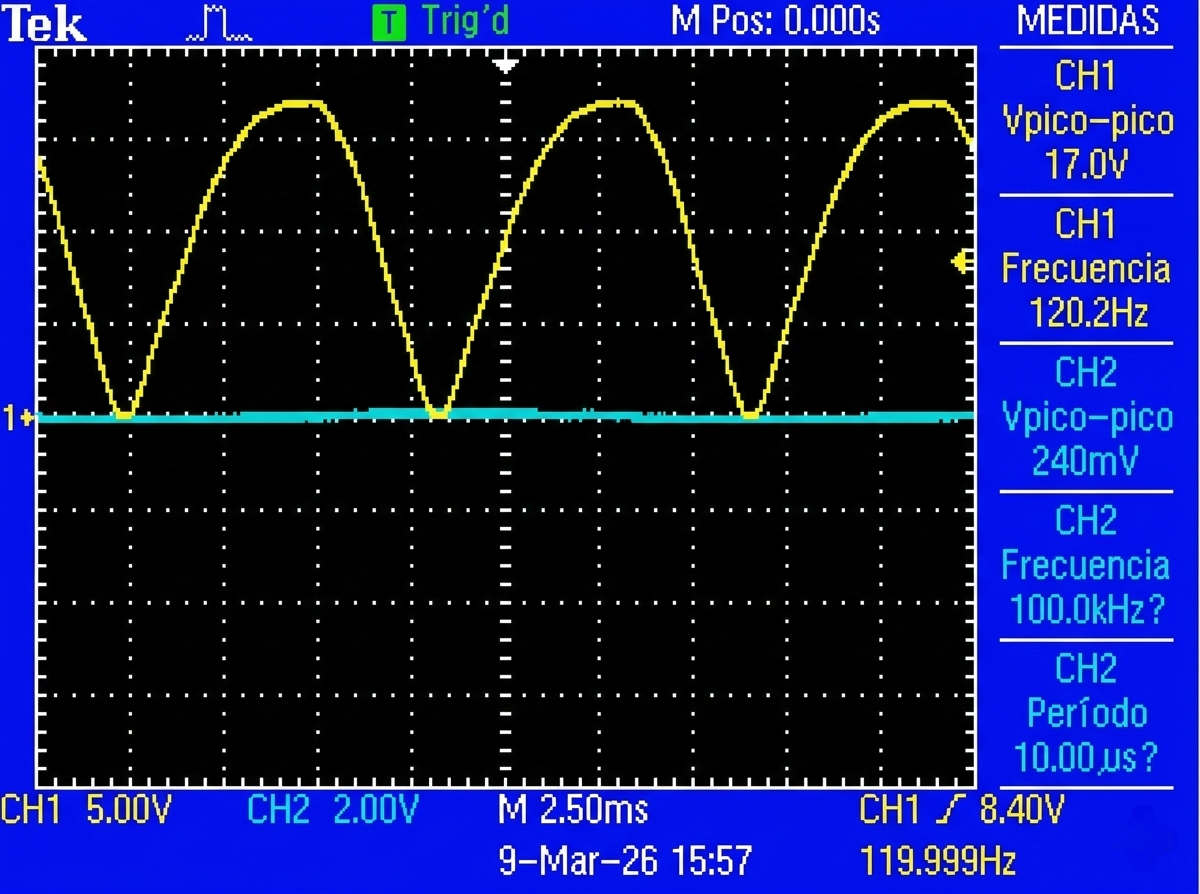
\includegraphics[width=0.45\textwidth]{IMAGENES/Rectificado.png} 
        \caption{Rectificación de Onda completa (120Hz).}
        \label{fig:Rectificado}
        \end{center}
        \end{figure}

        Entonces, la expresión que define la capacitancia queda determinada con los siguientes valores:
        \[
        C = \frac{0.758}{120(1.577)} = 4005.49\,\mu F
        \]

        El valor más cercano en el mercado es de:
        \[
        C=4700\mu F
        \]
        \subsection{Valores Reales.}
        Con los cálculos anteriores logramos definir los componentes a utilizar basándonos en la disponibilidad del mercado, entonces ahora obtendremos los valores reales esperados en práctica con los componentes seleccionados.
        \[
        I_R = \frac{V}{R} = \frac{9}{18} = 500\,mA
        \]
        Considerando el valor de la resistencia real a utilizar, podemos encontrar el valor de la corriente que circulara por el circuito integrado, que es de 500mA, lo cuál nos deja un gran margen respecto a los valores máximos y mínimos 
        que indica el fabricante.

        \[
        P_R = (9)(500 \times 10^{-3}) = 4.5\,W 
        \]

        \[
        \quad \text{(por seguridad debe ser el doble)}
        \]

        \[
        I_{\text{carga total}} = I_{CI} + I_{\text{control}} 
        = 8\,mA + 500\,mA = 508\,mA 
        \]

        \[
        V_r = \frac{0.508}{120(0.0047)} \approx 0.9007\,V_{pp} 
        \]
        El valor del voltaje de rizo queda comprobado con lo medido del osciloscopio, recordemos que la función del capacitor es "Linealizar" la señal de salida, esto se logra debido a que al capacitor no le da tiempo de cargarse o descargarse
        por lo que en los intervalos de tiempo donde la onda sinuidal natural del transformador varía (disminuye o aumenta) es donde el capacitor se descarga formando "rampas en esos intervalos". Lo anterior queda mejor descrito con la siguiente imagen:

        \begin{figure}[H]%[!ht]
        \begin{center}
        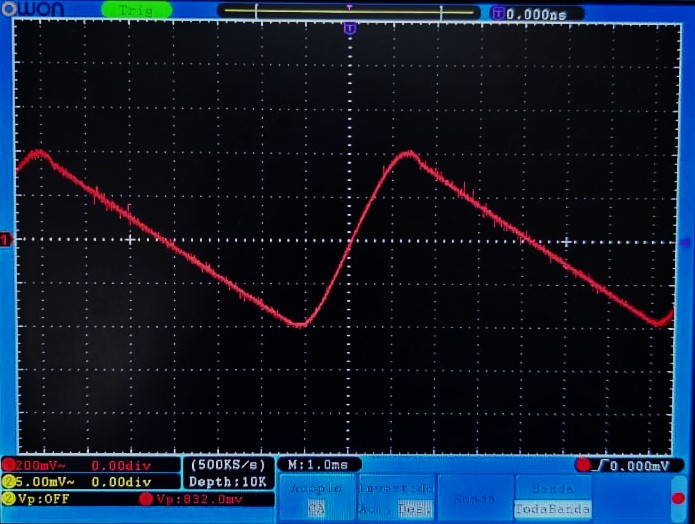
\includegraphics[width=0.45\textwidth]{IMAGENES/Voltaje_rizo.jpeg} 
        \caption{Voltaje Rizo.}
        \label{fig:VoltajeRizo}
        \end{center}
        \end{figure}

        El $V_R$ medido en osciloscopio fue de 0.840V, lo cuál se aproxima a lo esperado en los cálculos, además de cumplir con el criterio de $V_R \leq 0.10 V_{cd}$
        Si bien el circuito integrado trabaja dentro del rango de corriente esperado, existe una pérdida significante de voltaje entre la entrada y salida del mismo, estamos hablando de que a la entrada el regulador
        recibe 18.22V, de los cuáles sólo 9V dará a la salida más los aproximados 2V de caída de tensión mínima que presenta el circuito integrado. Todo ese voltaje se desprende en 
        forma de calor, por lo que es ncesario calcular y adquirir disipadores para incrementar el tiempo de trabajo de la fuente.

        \begin{itemize}
            \item $T_A$ = 25°C
            \item $T_j{max}$ = 100°C (recomendable)
            \item $\theta_{jc}$ = 5 °C/W.
            \item $\theta_{cs}$ = 0.5 °C/W
    \end{itemize}
        \[
        P_{CI} = (18.22 - 9)(0.508) = 4.68\,W
        \]

        \[
        T_J = T_A + P_D(\theta_{JC} + \theta_{CS} + \theta_{SA})
        \]

        \[
        \theta_{SA} = \frac{100 - 25}{4.68} - 5 - 0.5 = 10.52\,^\circ C/W
        \]

    \subsection{Resultados.}
    Una vez construido el circuito en físico se procedió a realizar mediciones de voltaje de salida para corroborar que todo funcionase de manera adecuada:
\begin{figure}[H]%[!ht]
\begin{center}
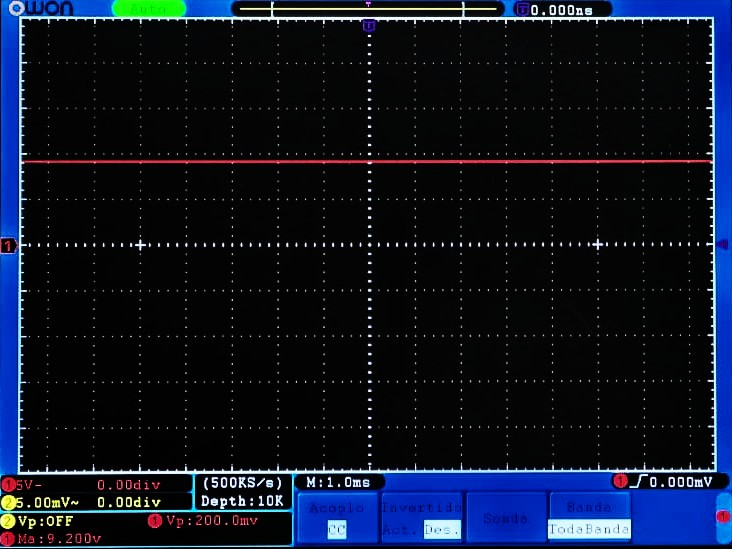
\includegraphics[width=0.45\textwidth]{IMAGENES/Osciloscopio_Positivo.jpeg} 
\caption{Medición de la terminal positiva.}
\label{fig:osc_pos}
\end{center}
\end{figure}
Como se logra apreciar, el voltaje de salida en la terminal positiva es aproximado a los 9V que se esperaban, es importante recalcar que el desarrollo de esta práctica considera
parámetros "complicados" para la fuente, pues para esto estamos utilizando la resistencia de carga mínima en la que la fuente puede operar de manera adecuada, sin exigir más corriente de la que el transformador
o el regulador pueden entregar. 

\begin{figure}[H]%[!ht]
\begin{center}
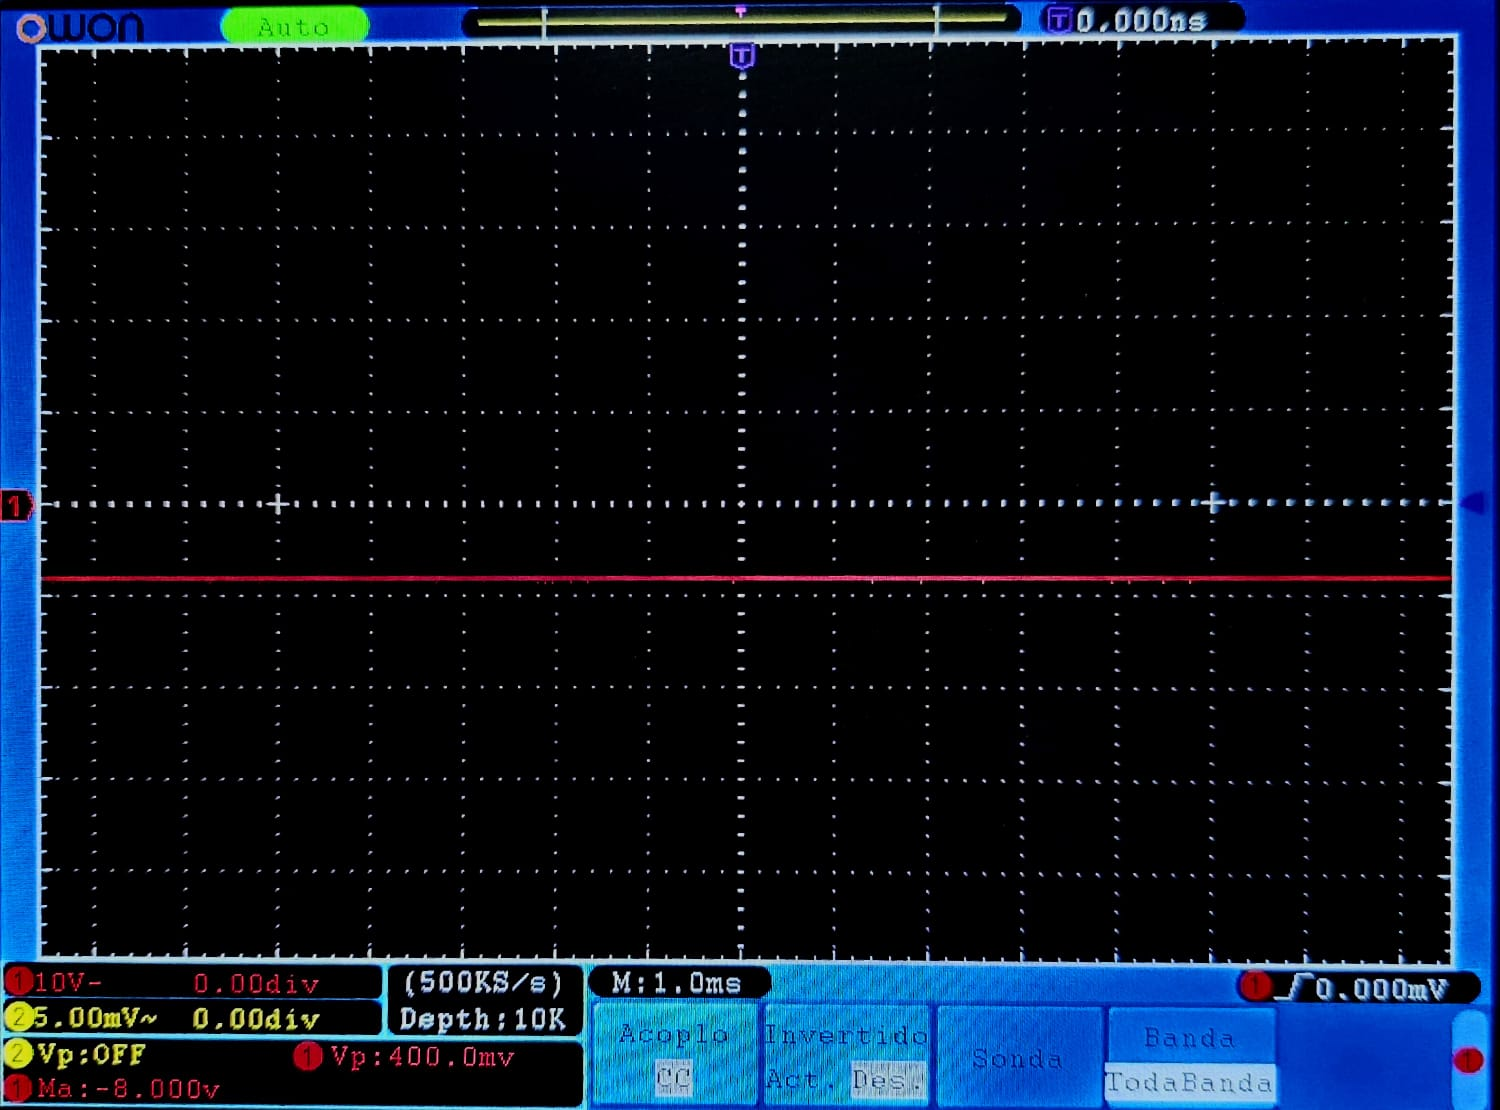
\includegraphics[width=0.45\textwidth]{IMAGENES/Osciloscopio_Negativo.jpeg} 
\caption{Medición de la terminal negativa.}
\label{fig:osc_neg}
\end{center}
\end{figure}
En este caso, la terminal negativa nos da un voltaje un poco por debajo de los -9V esperados, esto se debe al debanado del transformador, ya que la corriente y tensión 
no se distribuyeron homogéneamente en cada una de las terminales por lo que pudimos observar que en un devanado teníamos mayor voltaje de entrada que en el otro debanado.

Para ambos casos se observa que el voltaje de salida es aproximadamente el esperado (9V). A continuación se muestran las mediciones realizadas 
con multímetro con el fin de reafirmar los valores obtenidos a la salida del regulador.
\begin{figure}[H]%[!ht]
\begin{center}
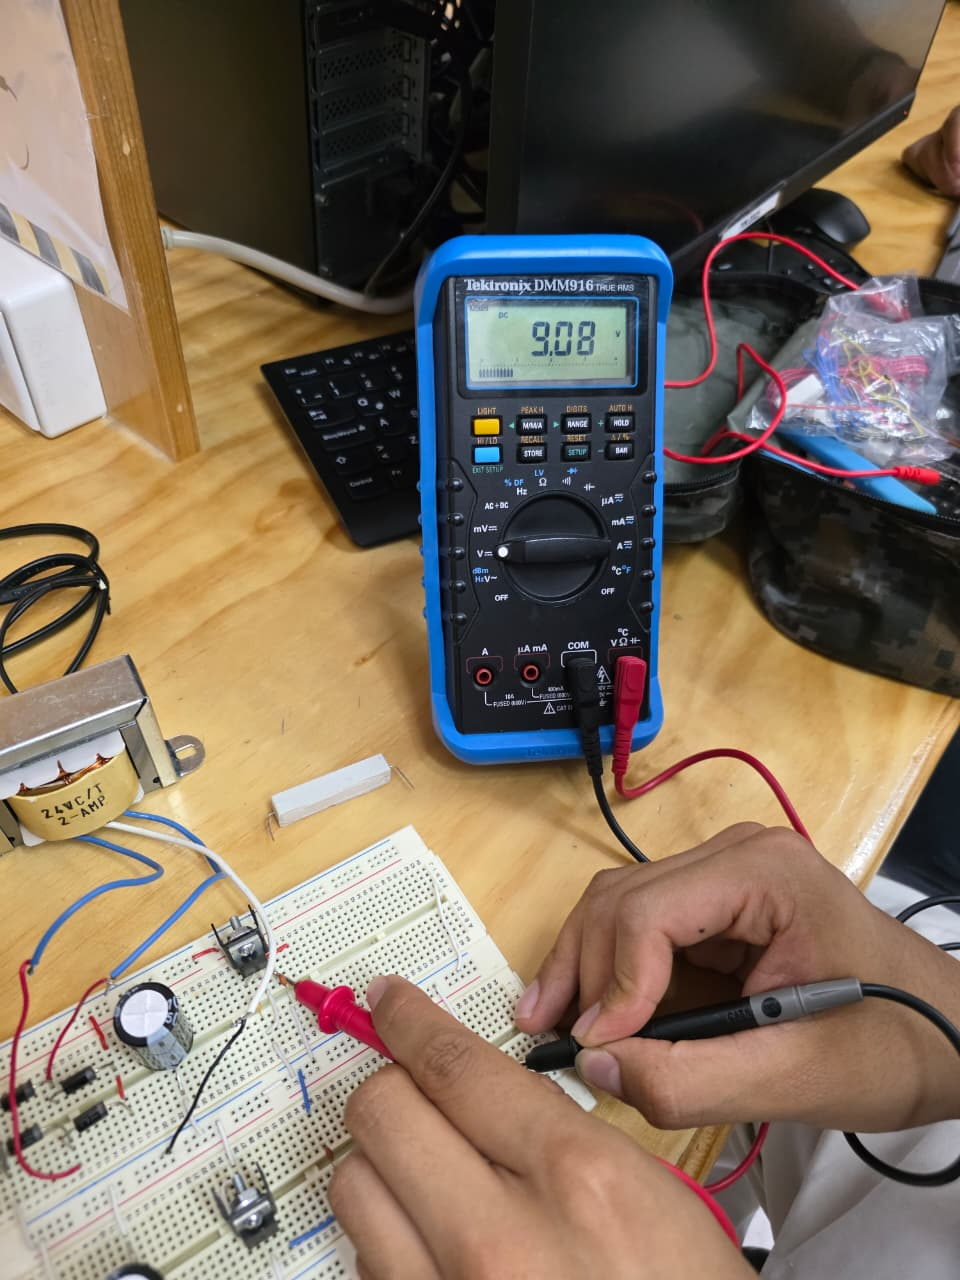
\includegraphics[width=0.45\textwidth]{IMAGENES/Multimetro_Positivo.jpeg} 
\caption{Medición en multímetro de la terminal positiva.}
\label{fig:mult_pos}
\end{center}
\end{figure}

\begin{figure}[H]%[!ht]
\begin{center}
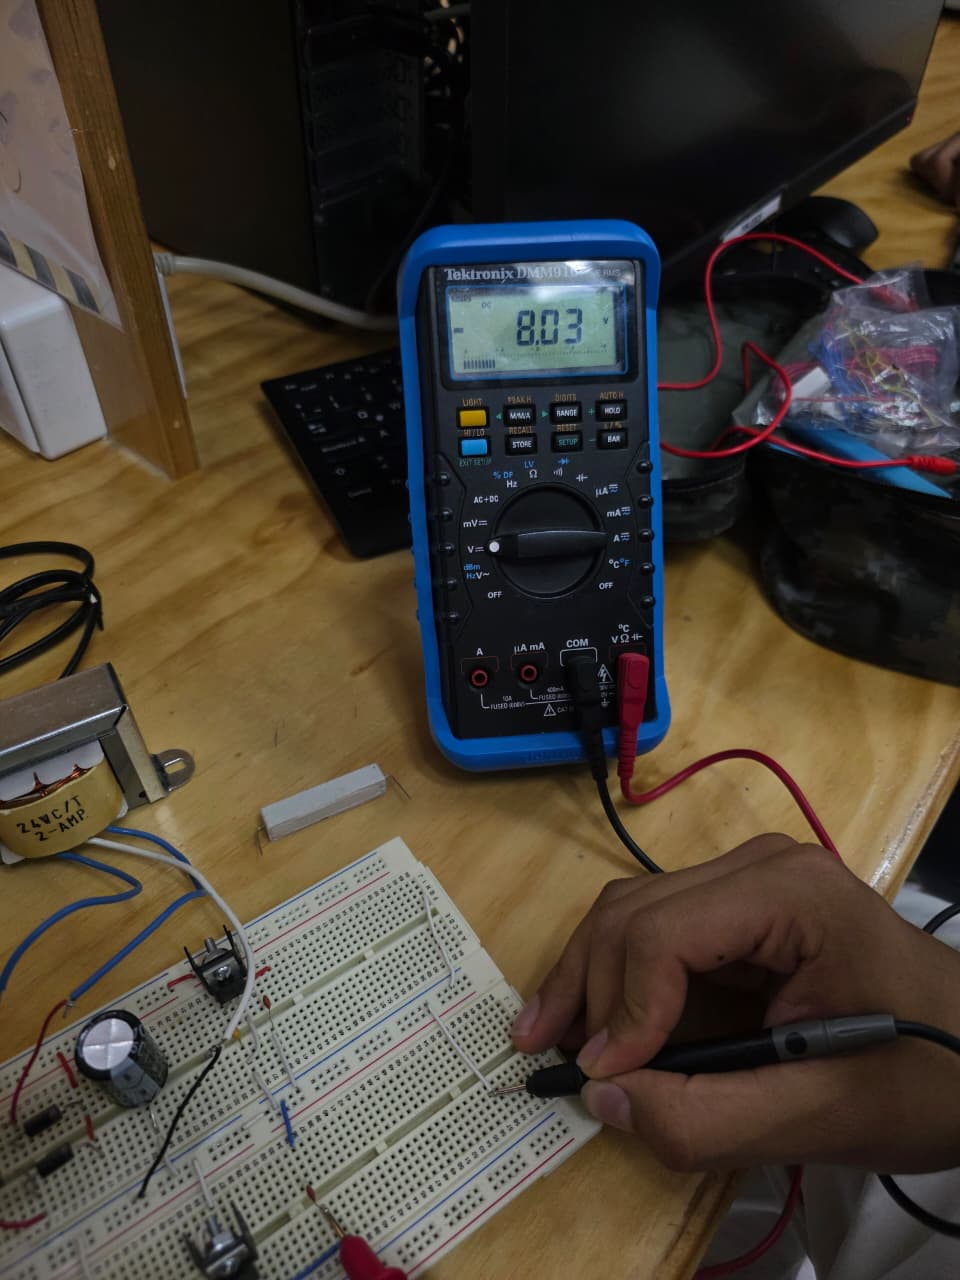
\includegraphics[width=0.45\textwidth]{IMAGENES/Multimetro_Negativo.jpeg} 
\caption{Medición en multímetro de la terminal negativa.}
\label{fig:mult_neg}
\end{center}
\end{figure}

A continuación se muestra en la tabla de manera resumida los valores obtenidos en la prueba de la fuente:
\begin{table}[H]
\centering
\small 
\begin{tabularx}{\columnwidth}{|c|X|X|X|X|}
\hline
\textbf{Parámetro} & \textbf{Valor Calculado} & \textbf{Valor Medido} & \textbf{Diferencia \%} \\ \hline
$V_{out}(+)$sin carga & 9V & 9V &   0\\ \hline
$V_{out}(+)$con carga & 9V & 9.6V &  6.67 \\ \hline
$V_{out}(-)$sin carga & -9V & -9V &    0 \\ \hline
$V_{out}(-)$con carga & -9V & -8.3V &     7.78  \\ \hline
$V_R$ & 0.9007V & 0.840V &     6.74 \\ \hline
\end{tabularx}
\caption{Tabla comparativa de resultados de la fuente bipolar lineal.}
\label{tablaComparativaFUENTE}
\end{table}

Donde la diferencia porcentual está definida como:
\[
\text{Error \%} = \frac{|\text{valor medido} - \text{valor calculado}|}{|\text{valor calculado}|} \times 100
\]

\section{Simulación}
Para esta sección nos basaremos en el circuito mostrado en la "Figura~\ref{fig:circuito_base}” para la simulación.
    \subsection{Valores Teóricos.}
    Para esta primera parte se analizarán los parmámetros de salida con los valores teóricos calculados con anterioridad.
        \begin{figure}[H]%[!ht]
        \begin{center}
        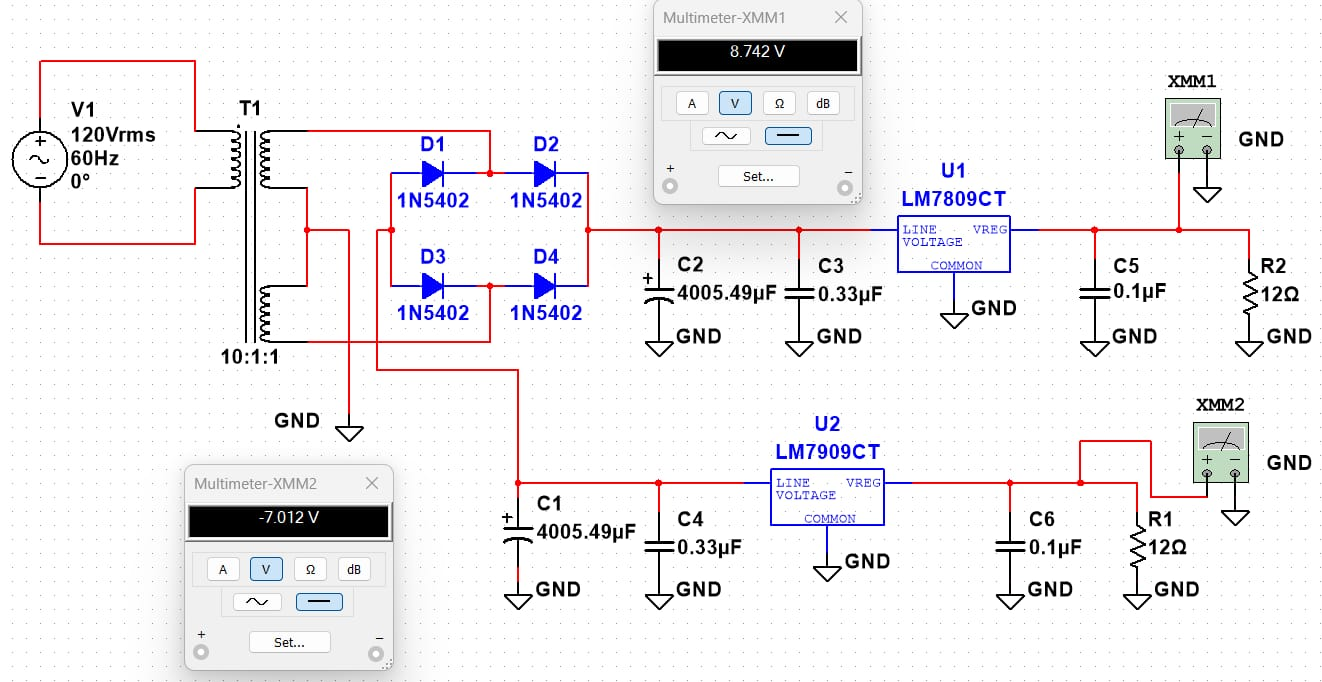
\includegraphics[width=0.45\textwidth]{IMAGENES/Simulacion_SalidaConCarga.jpeg} 
        \caption{Simulacion con valores teóricos a la salida con carga.}
        \label{fig:sim_teo_carga}
        \end{center}
        \end{figure}

        \begin{figure}[H]%[!ht]
        \begin{center}
        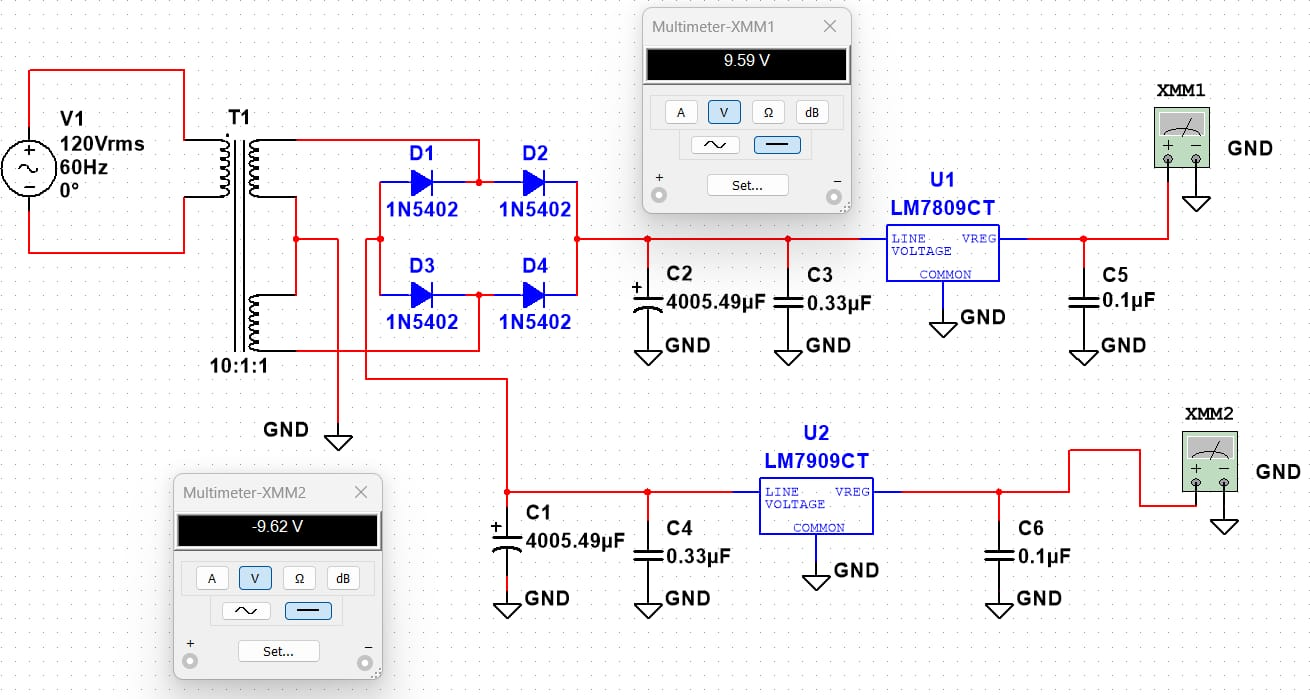
\includegraphics[width=0.45\textwidth]{IMAGENES/Simulacion_SalidaSinCarga.jpeg} 
        \caption{Simulacion con valores teóricos a la salida sin carga.}
        \label{fig:sim_teo_nocarga}
        \end{center}
        \end{figure}

        \begin{figure}[H]%[!ht]
        \begin{center}
        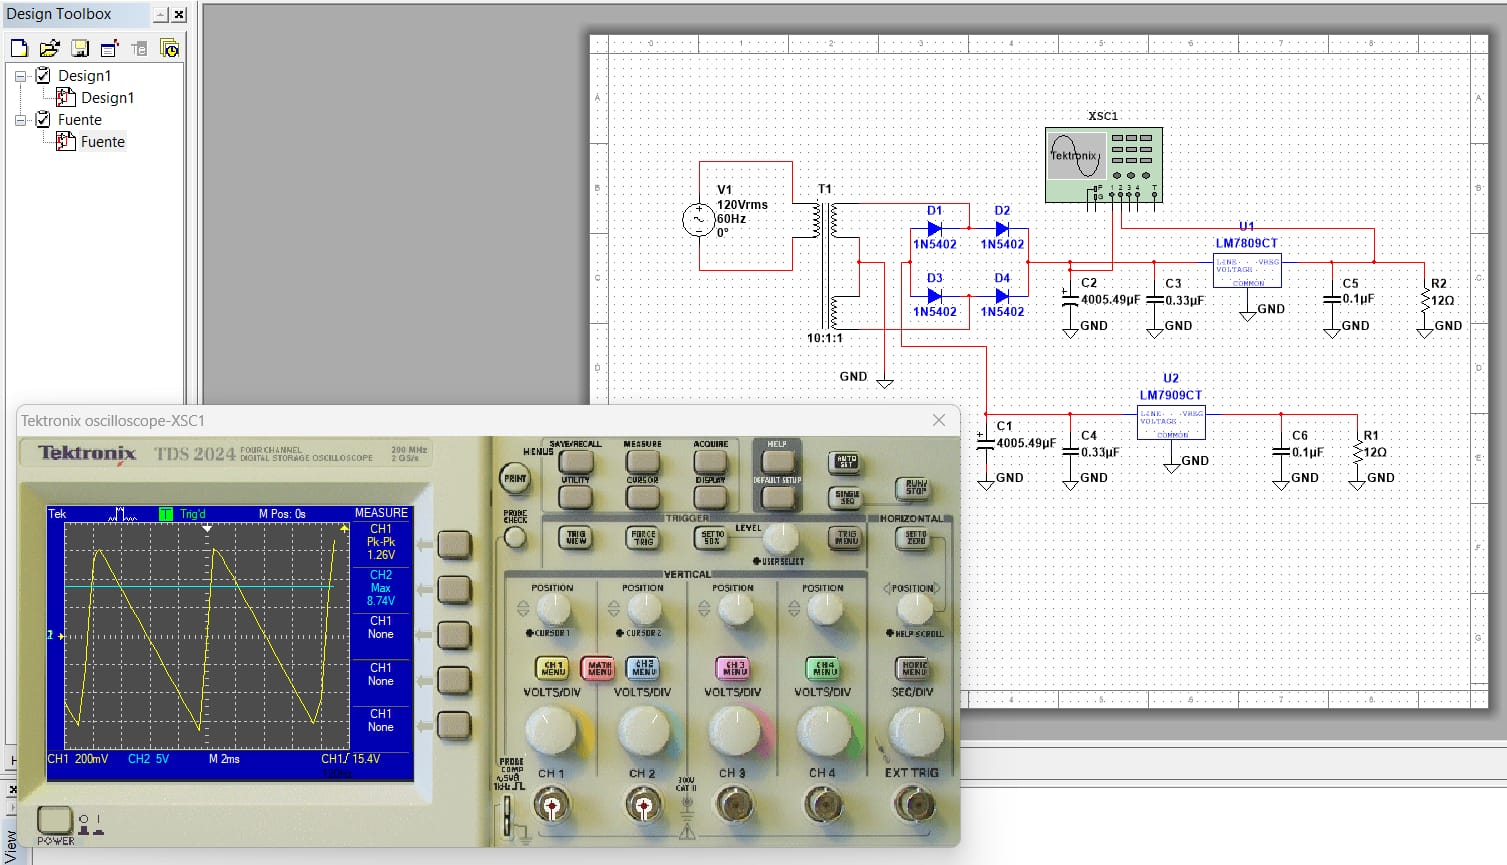
\includegraphics[width=0.45\textwidth]{IMAGENES/Simulacion_rizo_teorico.jpeg} 
        \caption{Simulacion con valores teóricos del voltaje de rizo.}
        \label{fig:sim_teo_rizo}
        \end{center}
        \end{figure}

    \subsection{Valores Reales.}
        \begin{figure}[H]%[!ht]
        \begin{center}
        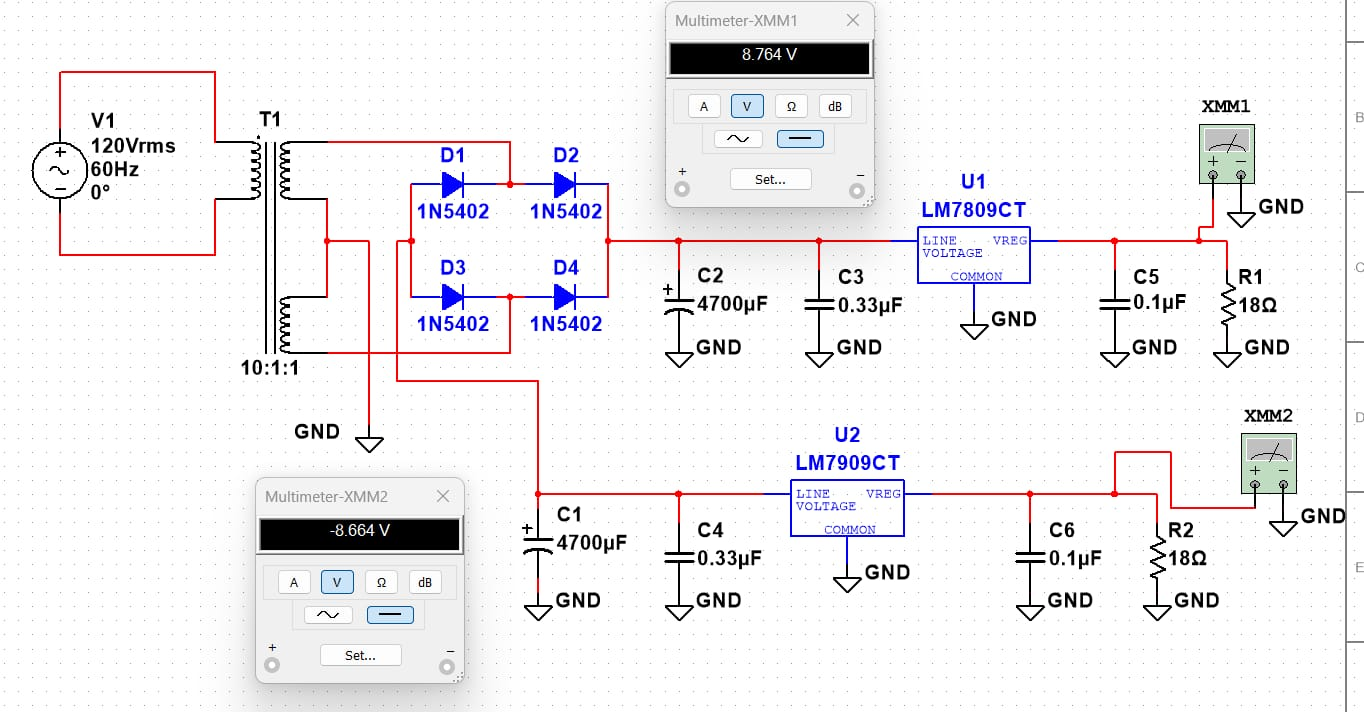
\includegraphics[width=0.45\textwidth]{IMAGENES/Simulacion_realSalidaConCarga.jpeg} 
        \caption{Simulacion con valores reales a la salida con carga.}
        \label{fig:sim_real_carga}
        \end{center}
        \end{figure}

        \begin{figure}[H]%[!ht]
        \begin{center}
        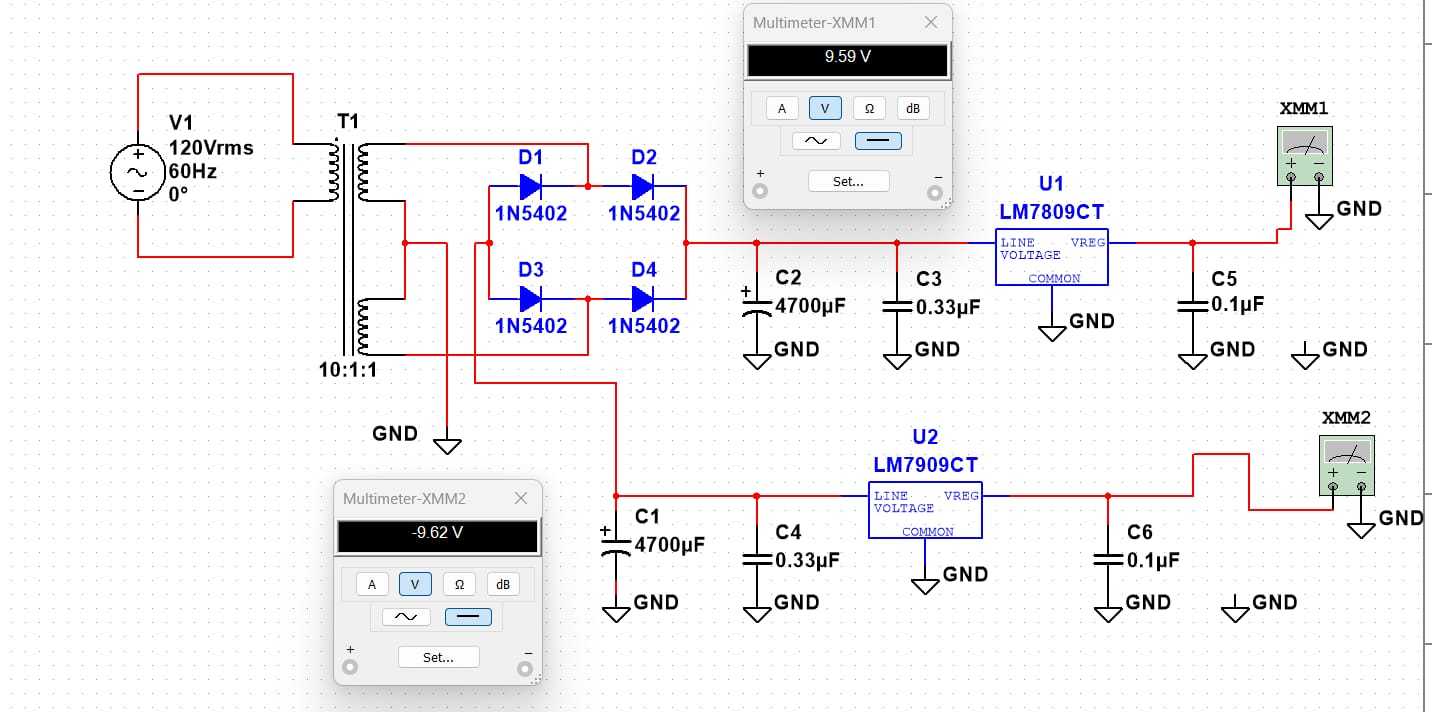
\includegraphics[width=0.45\textwidth]{IMAGENES/Simulacion_realSalidaSinCarga.jpeg} 
        \caption{Simulacion con valores reales a la salida sin carga.}
        \label{fig:sim_real_nocarga}
        \end{center}
        \end{figure}

        \begin{figure}[H]%[!ht]
        \begin{center}
        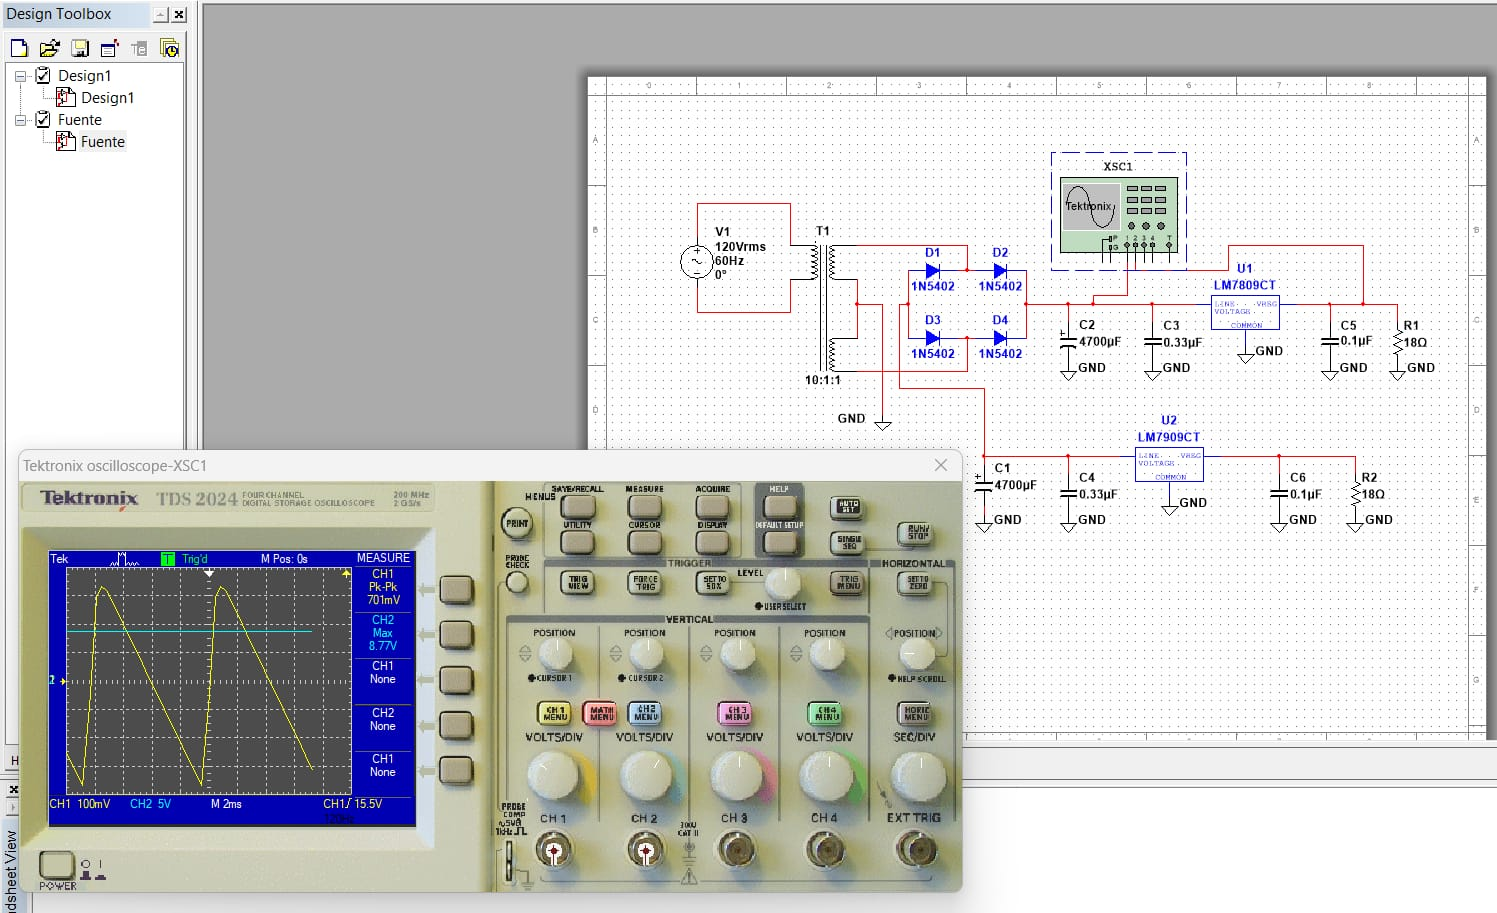
\includegraphics[width=0.45\textwidth]{IMAGENES/Simulacion_rizo_real.jpeg} 
        \caption{Simulacion con valores reales del voltaje de rizo.}
        \label{fig:sim_real_rizo}
        \end{center}
        \end{figure}
\section{Conclusiones}
\begin{itemize}
    \item \textbf{Flores Cornejo Gustavo Mauricio.}
    \newline 
    El desarrollo de este proyecto fue algo complicado en un principio, pues diseñar un circuito basándonos únicamente en parámetros de salida deseados no es lo que normalmente desarrollamos en ejercicios y otras prácticas. Además, para este proyecto fue necesario tener varios parámetros a considerar que de no prestar la suficiente atención afectaban directamente al comportamiento de la fuente.
    También fue un tema complicado la cuestión de disipación de calor, mantener al circuito integrado estable para soportar el tiempo de duración de la evaluación fue complicado considerando que la variación de los resultados dependía en gran medida a la temperatura de los componentes. El proyecto me ayudó a comprender y participar en el funcionamiento de una fuente lineal, además de poder visualizar vario elementos en uno solo 
    (diodos como rectificadores, capacitor como filtro y regulador como ajuste a voltaje de salida).
    En general resulta una muy buena práctica para poner en práctica la teoría conocida de los elementos que la componen por separado, además de tener que investigar otras consideraciones que no tenías en cuenta antes, como lo es la variación térmica.
    \newline 
    \item \textbf{Muñoz Reyes Arturo Yabet.}
    \newline El desarrollo de la presente fuente bipolar lineal representó un desafío técnico significativo, al transicionar de la resolución de ejercicios teóricos hacia un diseño basado estrictamente en parámetros de salida predefinidos. Durante la etapa experimental, se evidenció que la estabilidad del sistema no depende únicamente del cálculo ideal de los componentes, sino de factores críticos de implementación, siendo la disipación térmica el obstáculo más complejo. Se determinó que la elevación de temperatura en los reguladores 78XX y 79XX afecta directamente la precisión de la tensión de salida, lo que subraya la importancia de una gestión térmica adecuada para mantener el punto de operación estable durante pruebas prolongadas. En conclusión, el proyecto permitió integrar de forma sistémica el comportamiento de semiconductores, filtros capacitivos y circuitos integrados, reforzando que un diseño exitoso requiere considerar variables físicas reales, como la variación térmica y las tolerancias de los componentes, más allá de las aproximaciones matemáticas convencionales.
    
    \item \textbf{Morales Vásquez Miguel Ehecatl.} 
    \newline El desarrollo de la fuente bipolar lineal representó una experiencia de gran valor tanto en el aspecto teórico como en la parte práctica, ya que permitió enfrentar un diseño real a partir de parámetros de salida previamente establecidos, alejándose de los ejercicios convencionales donde la mayoría de las variables suelen estar definidas desde el inicio. Durante el proceso se comprobó que el correcto funcionamiento de la fuente no depende únicamente de los cálculos matemáticos, sino también de factores físicos que influyen directamente en el desempeño del circuito, como la disipación térmica, las tolerancias de los componentes y la estabilidad de los reguladores de voltaje. La temperatura en los circuitos integrados 78XX y 79XX fue uno de los aspectos más críticos, debido a que su incremento afectaba la regulación y precisión de la salida, haciendo indispensable una adecuada gestión térmica mediante disipadores y una correcta selección de componentes. Asimismo, el proyecto permitió integrar de forma práctica el funcionamiento conjunto de diodos rectificadores, capacitores de filtrado, transformador y reguladores lineales, logrando una visión más completa del comportamiento de una fuente de alimentación. En conclusión, esta práctica reforzó la importancia de considerar no solo el diseño ideal, sino también las condiciones reales de operación, consolidando conocimientos fundamentales de electrónica de potencia y diseño de fuentes lineales.

\end{itemize}



% if have a single appendix:
%\appendix[Proof of the Zonklar Equations]
% or
%\appendix  % for no appendix heading
% do not use \section anymore after \appendix, only \section*
% is possibly needed

% use appendices with more than one appendix
% then use \section to start each appendix
% you must declare a \section before using any
% \subsection or using \label (\appendices by itself
% starts a section numbered zero.)
%


\appendices
\section{Evidencias}
    \begin{figure}[H]%[!ht]
    \begin{center}
    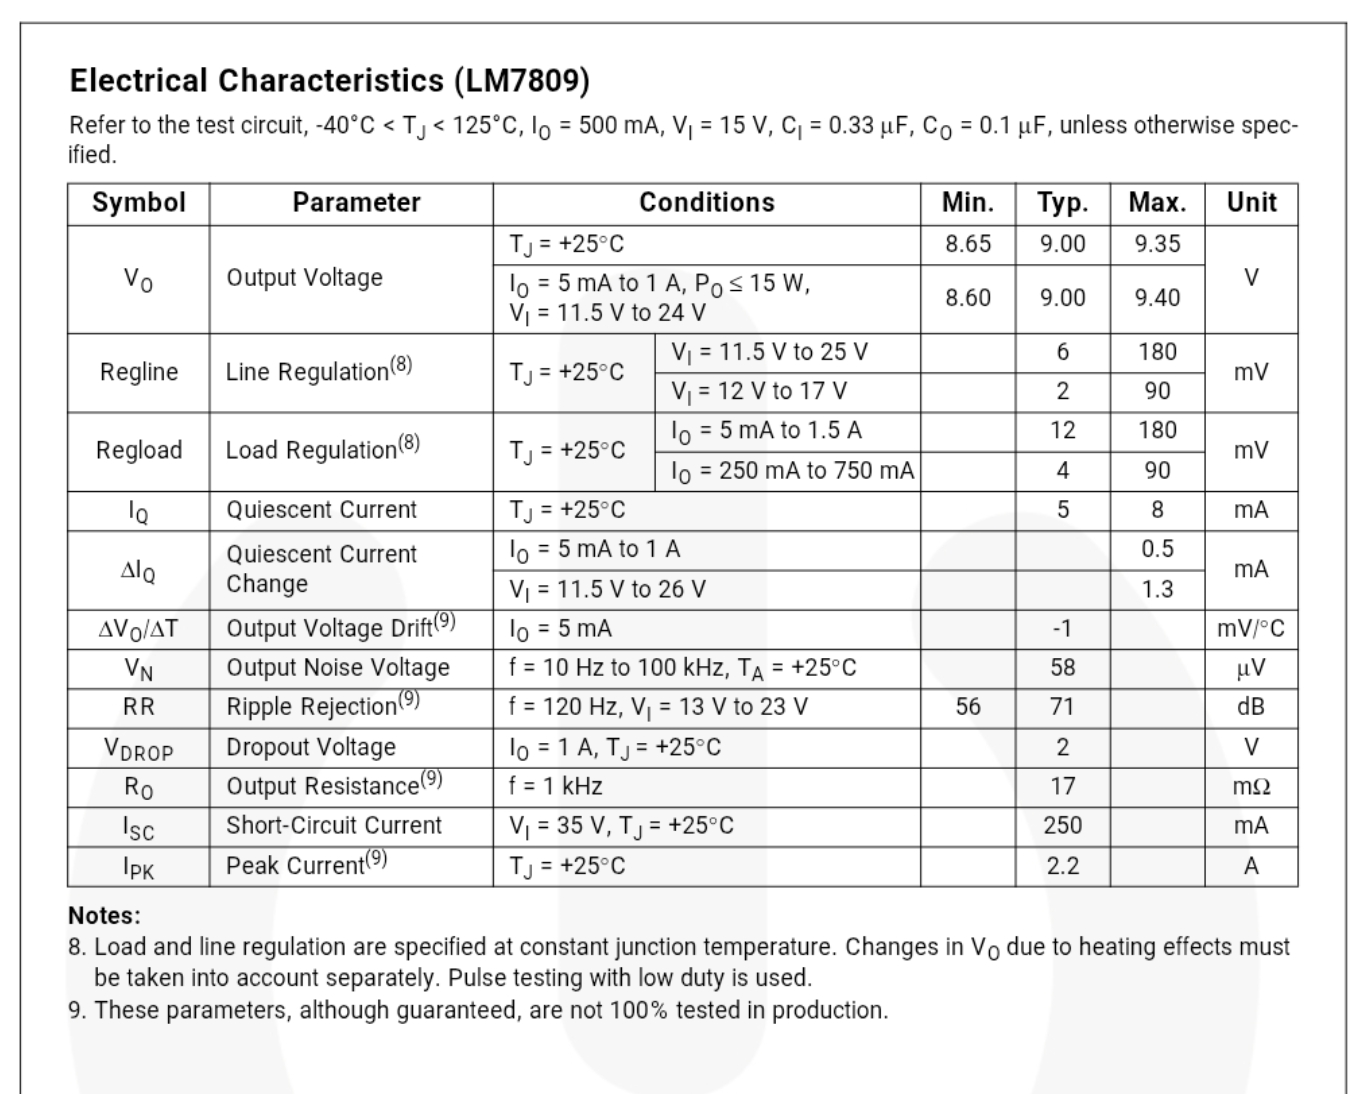
\includegraphics[width=0.45\textwidth]{IMAGENES/Datasheet_LM7809.jpeg} 
    \caption{Datasheet del circuito integrado LM7809.}
    \label{fig:datasheet_LM7809}
    \end{center}
    \end{figure}

    \begin{figure}[H]%[!ht]
    \begin{center}
    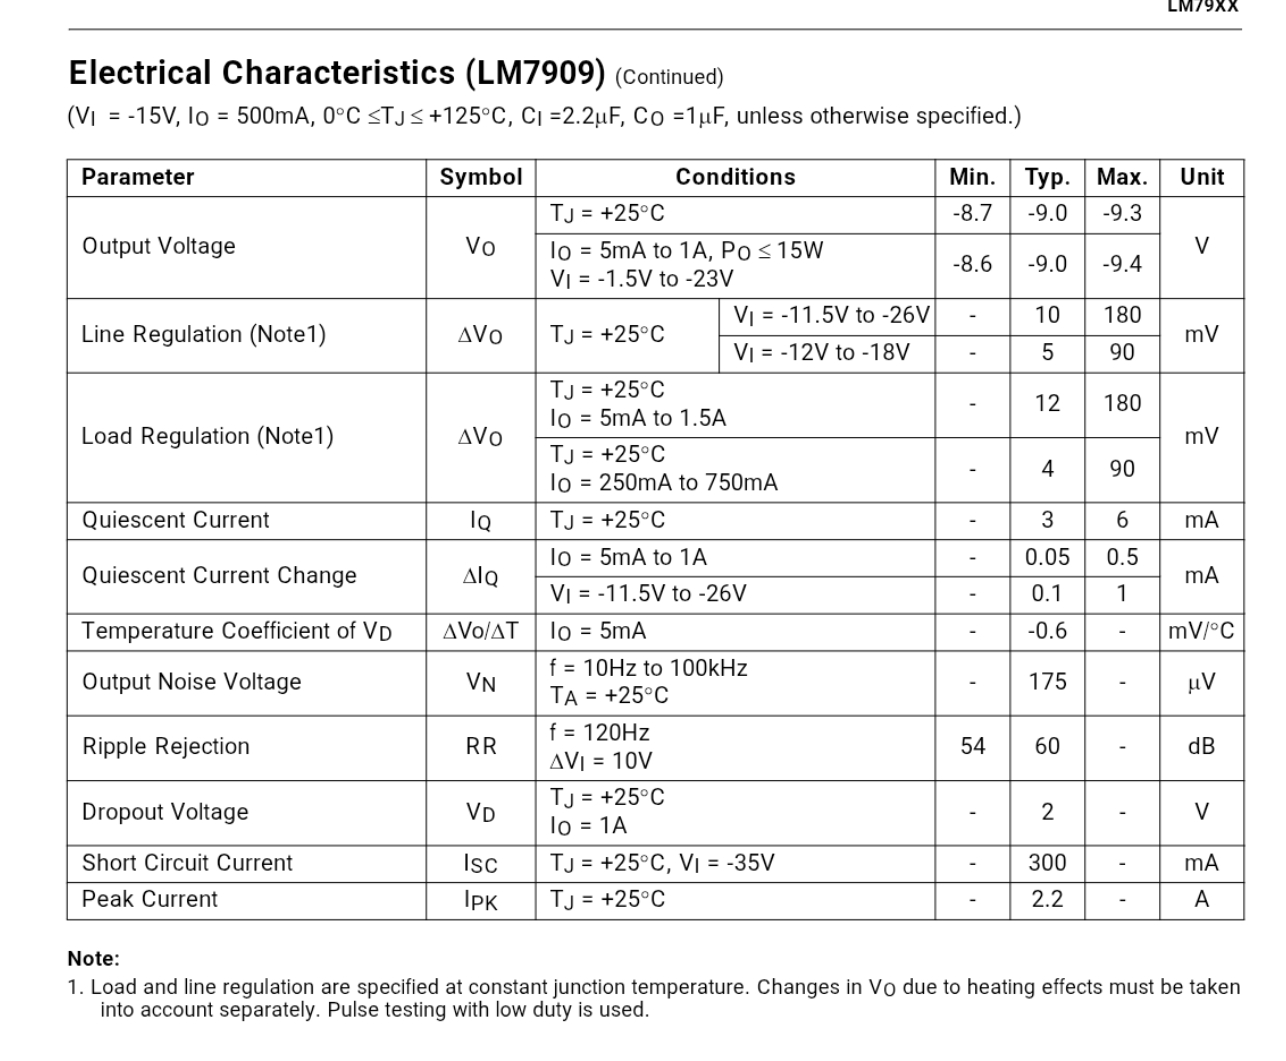
\includegraphics[width=0.45\textwidth]{IMAGENES/Datasheet_LM7909.jpeg} 
    \caption{Datasheet del circuito integrado LM7909.}
    \label{fig:datasheet_LM7909}
    \end{center}
    \end{figure}

    \begin{figure}[H]%[!ht]
    \begin{center}
    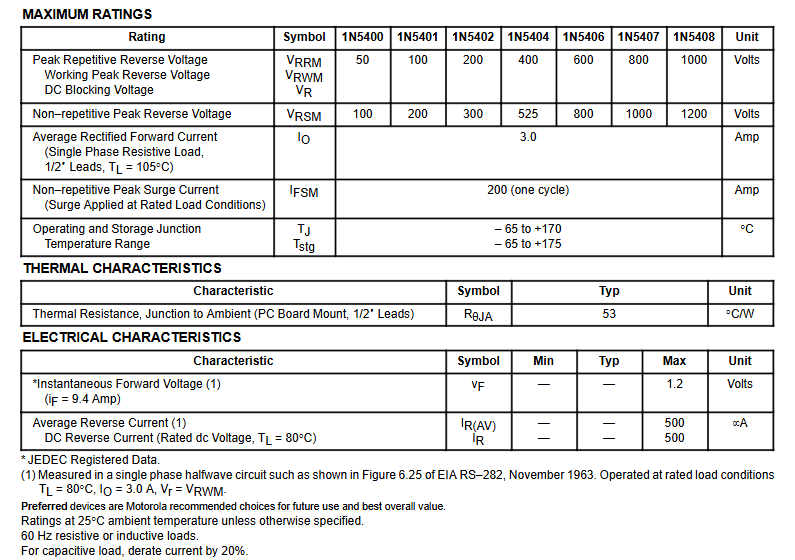
\includegraphics[width=0.45\textwidth]{IMAGENES/Datasheet_1N5402.png} 
    \caption{Datasheet del diodo 1N5402.}
    \label{fig:datasheet_1N5402}
    \end{center}
    \end{figure}

    \begin{figure}[H]%[!ht]
    \begin{center}
    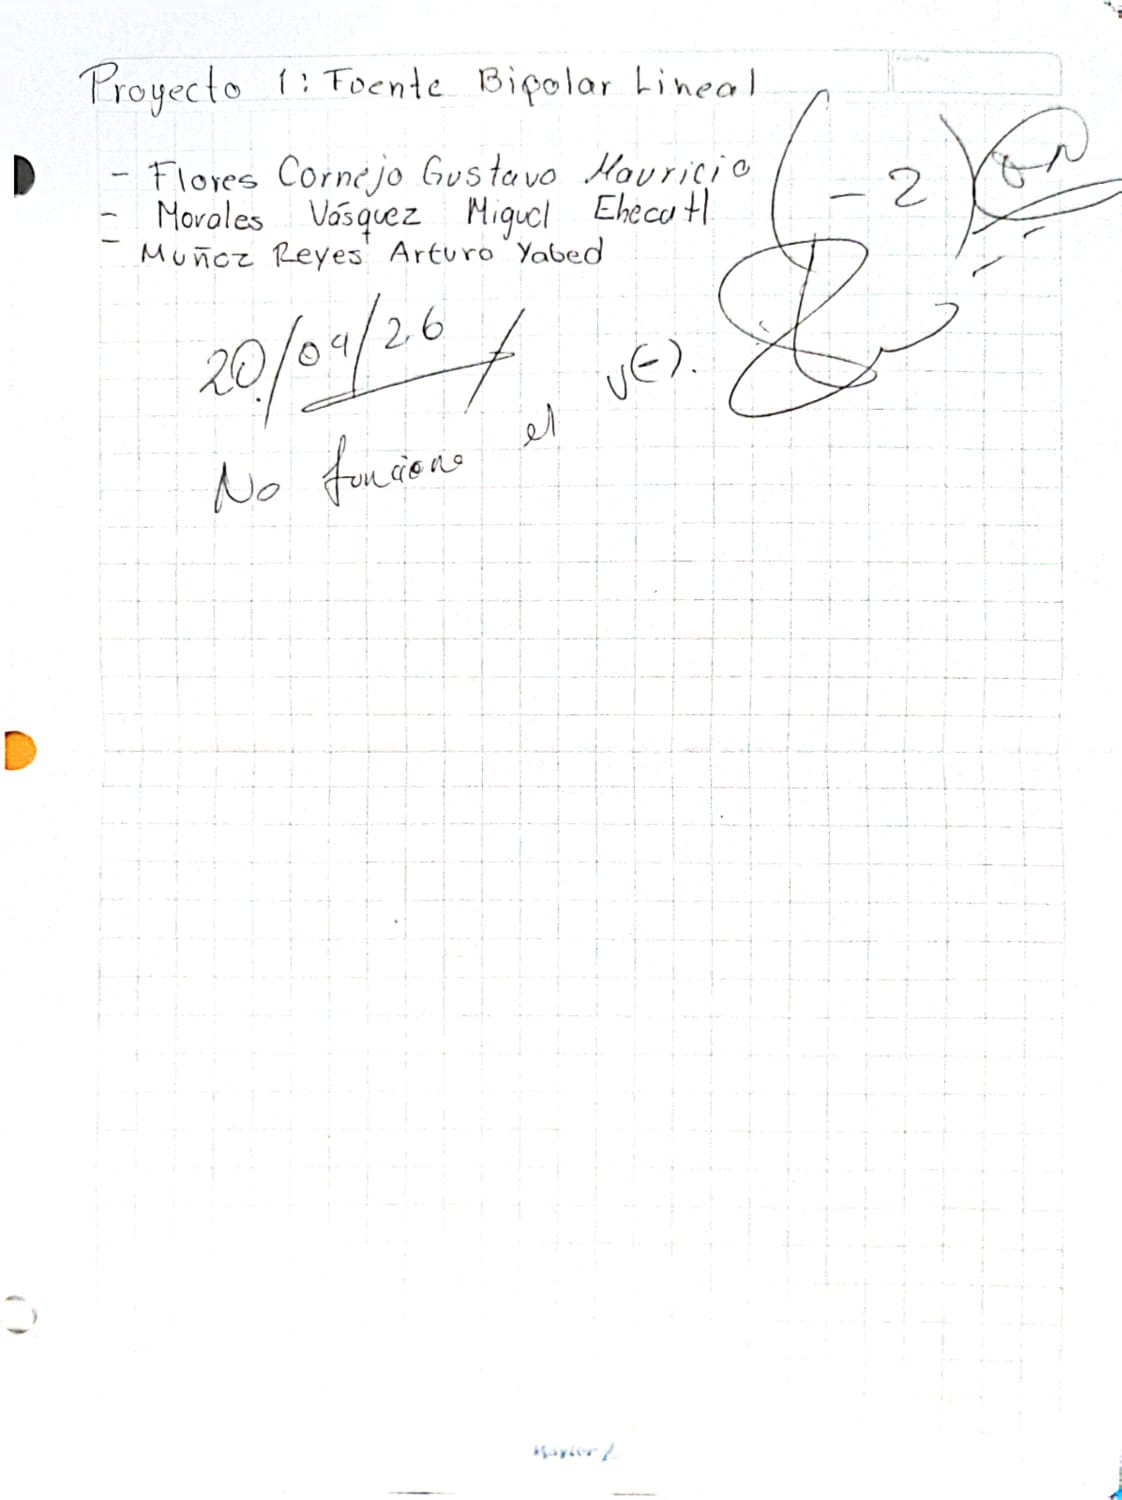
\includegraphics[width=0.45\textwidth]{IMAGENES/Evidencia.jpeg} 
    \caption{Evidencia de entrega.}
    \label{fig:evidencia}
    \end{center}
    \end{figure}




% references section

% can use a bibliography generated by BibTeX as a .bbl file
% BibTeX documentation can be easily obtained at:
% http://mirror.ctan.org/biblio/bibtex/contrib/doc/
% The IEEEtran BibTeX style support page is at:
% http://www.michaelshell.org/tex/ieeetran/bibtex/
%\bibliographystyle{IEEEtran}
% argument is your BibTeX string definitions and bibliography database(s)
%\bibliography{IEEEabrv,../bib/paper}
%
% <OR> manually copy in the resultant .bbl file
% set second argument of \begin to the number of references
% (used to reserve space for the reference number labels box)

%use following command to generate the list of cited references

\printbibliography

\begin{thebibliography}{00}
\bibitem{boylestad}
R. L. Boylestad and L. Nashelsky, \textit{Electronic Devices and Circuit Theory}, 10th ed. Upper Saddle River, NJ, USA: Prentice Hall, 2009.

\bibitem{1N4001}
onsemi, ``1N4001 -- 1.0 A Standard Recovery Rectifier,'' Datasheet, 2023. [Online]. Available: https://www.onsemi.com/pdf/datasheet/1n4001-d.pdf. [Accessed: Feb. 24, 2026].

\bibitem{1N4148}
onsemi, ``1N4148 -- Small Signal Switching Diode,'' Datasheet, 2023. [Online]. Available: https://www.onsemi.com/pdf/datasheet/1n4148-d.pdf. [Accessed: Feb. 24, 2026].
\end{thebibliography}

% that's all folks
\end{document}